\section{Cognitive Architectures}
\label{sec:cogarch}
Cognitive architectures are architectures that base themselves on some model of
human cognition. There are several competing models of cognition, and one of
the most recent and well-supported is the Global Workspace Theory.

One area that haven't been as well explored in relation to RTSes in general and
StarCraft in particular, is cognitive architectures.
There has been some research done into implementing cognitive models for use in
first-person shooter games, but not into real-time strategy games. There
currently have been no attempts at utilizing cognitive models for playing
Starcraft: BroodWar. It would seem intuitive that real-time strategy games,
which have been considered a relatively hard problem to solve in a human-like
fashion, would benefit from using models based on our understanding of human
cognition. It is also peculiar that while so much work has been put into making
believable game-playing agents, very little focus has been on reproducing the
effects of cognitive models.  Arrabales et al put forth that this is perhaps
because of poor understanding within the field of classical AI of research into
cognition\cite{arrabales2009gamechars}.

\subsection{Global Workspace Theory}

\begin{figure}[h!tb]
\centering
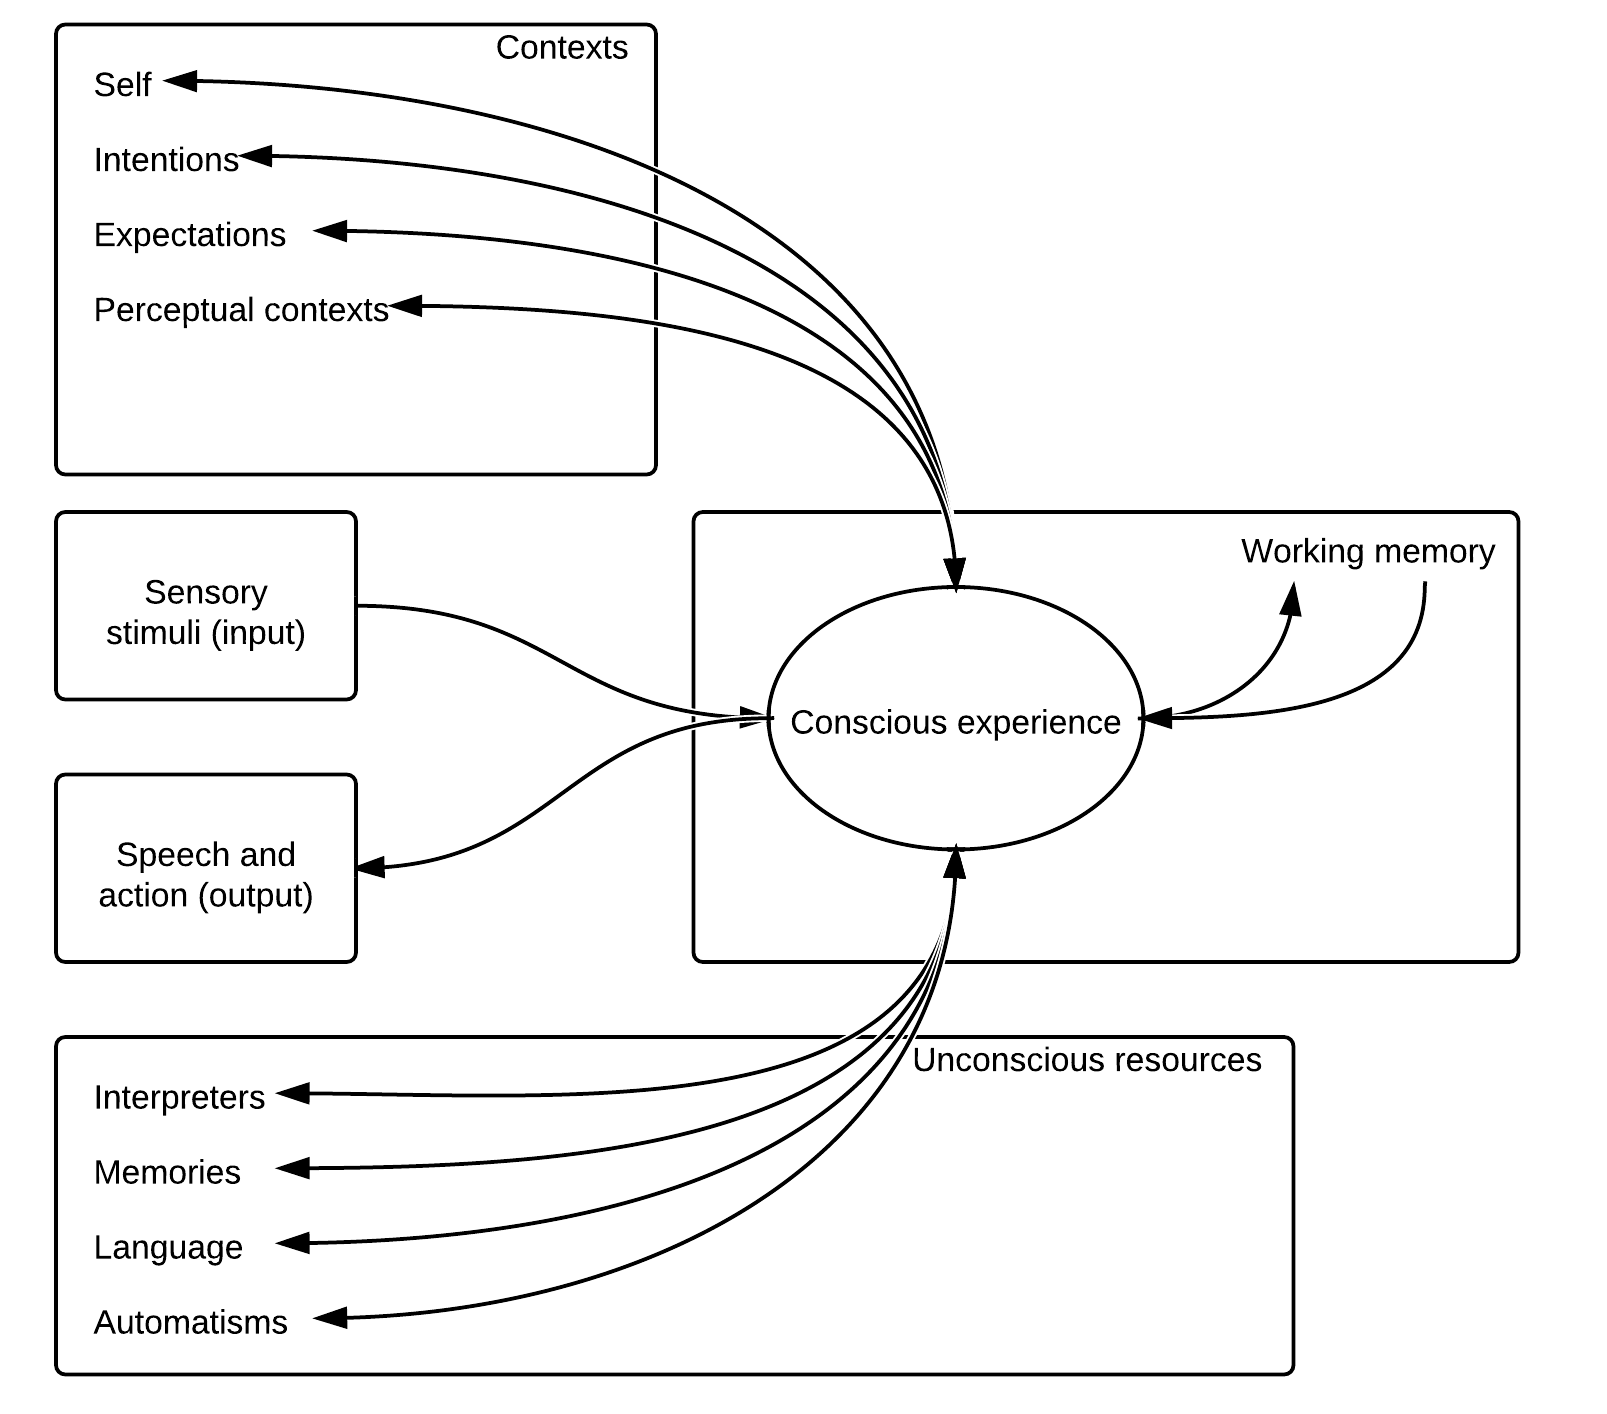
\includegraphics[scale=1.0]{graphics/globalworkspace.png}
\caption{A schematic of the Global Workspace theory\cite{baars2005gwt}}
\label{fig:gwt}
\end{figure}

Global Workspace Theory is a model of cognition that is very well supported by
experimental data, and is one of the most widely accepted
models.\cite{dehaene2001towards} It has been used to implement processes that
imitate human decision making (for example for solving the problem of assigning
people to jobs in the US Navy).\cite{baars2005gwt}\cite{franklin2003interacting}

It is based around an understanding of the brain as a set of many independently
processing modules, working together by utilizing a shared workspace (hence the
``global workspace''). Every ``cognitive cycle'' all the
processes compete for attention, and a single one gets the
proverbial spotlight shone upon it.\cite{baars2005gwt}

There have been several implementations of GWT for different domains and
approaches, for example the LIDA (``Learning IDA'')
model\cite{franklin2007lida}, or the CERA-CRANIUM
architecture\cite{arrabales2009ceracranium}.

See figure \ref{fig:gwt} for an overview of the theory.

\subsection{Cognitive Models in Game AIs}
There have been several more or less successful attempts at implementing models
of cognition into game-playing agents. One of the more recent ones is
CERA-CRANIUM. One of the reasons for using computer games for experiments wrt.
high-level artificial intelligence is that the characteristics of computer
games lend themselves to this, by eliminating noise and uncertainty, and
providing a more or less realistic simulated environment.


\subsection{CERA-CRANIUM}
\begin{figure}[h!tb]
\centering
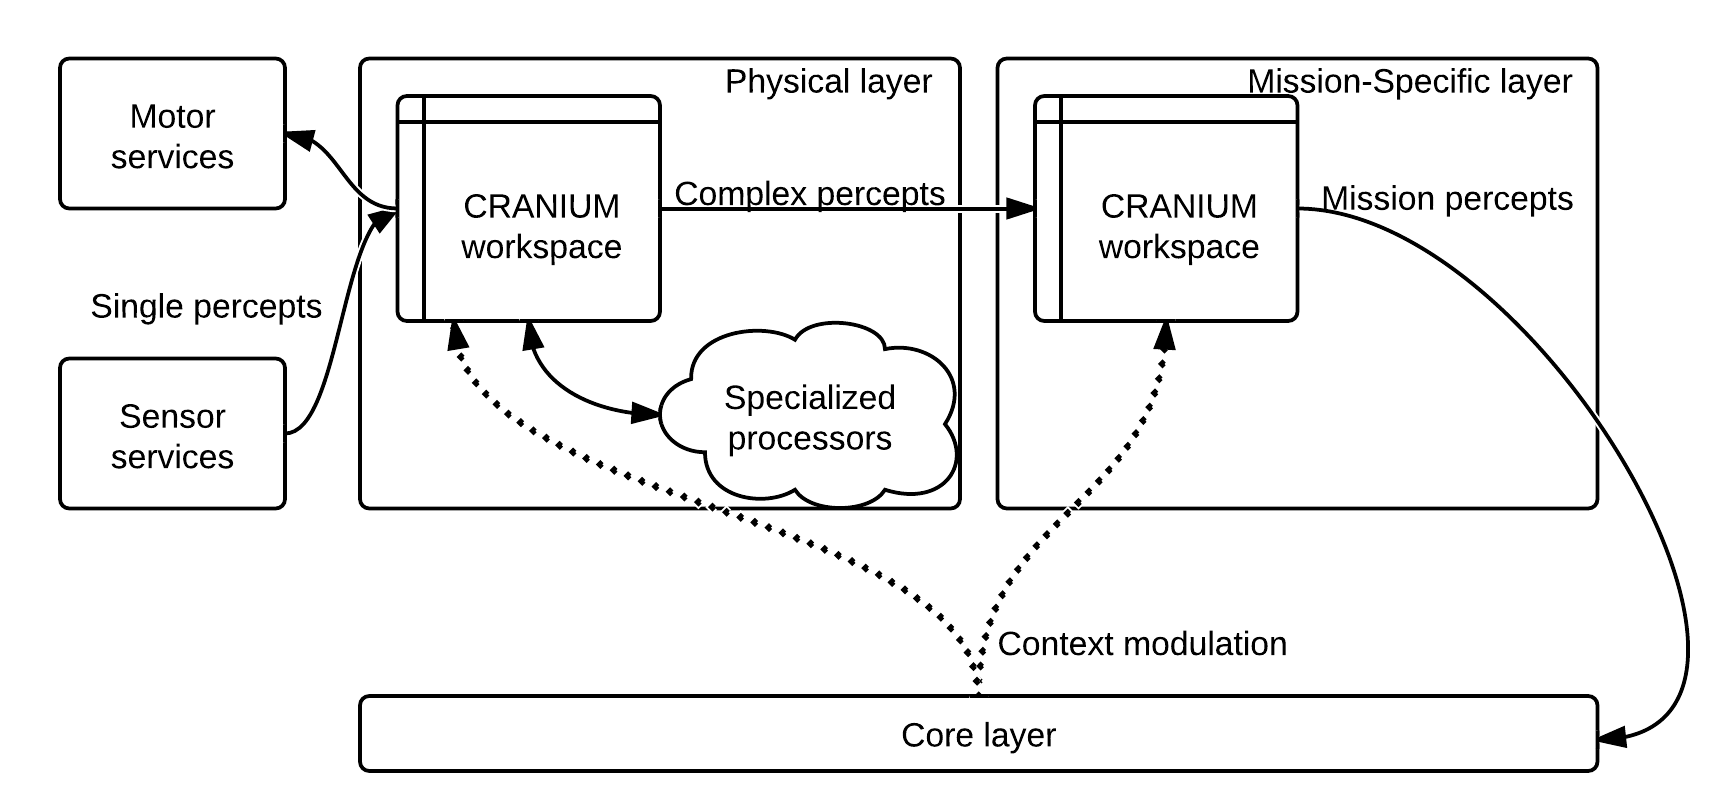
\includegraphics[scale=1.0]{graphics/ceracranium.png}
\caption{A schematic of CERA-CRANIUM\cite{arrabales2009ceracranium}}
\label{fig:ceracranium}
\end{figure}

CERA-CRANIUM intends to implement a general architecture for agents based on
various cognitive architectures, and not tied to any specific model of
cognition. It has already been used to implement a bot that plays Unreal
Tournament 2004 (a first-person shooter game) using a model based on the Global
Workspace Theory, as well as a robot for mapping out an unknown environment.
\cite{arrabales2009ceracranium}

It is based on two major modules:
\begin{description}
 \item [CRANIUM] (Cognitive Robotics Architecture Neurologically Inspired
Underlying Manager) is a tool to create and manage a large amount of
simultanous processes interacting through a shared workspace.
 \item [CERA] (Conscious and Emotional Reasoning Architecture)
 utilizes CRANIUM to create a dynamic control architecture structured in
layers, based on computational models of consciousness.
\end{description}

Figure \ref{fig:ceracranium} presents a rough overview of how the architecture
is structured, and in the following subsections we will present a more
detailed look at how it works and how the various parts interoperate.

\subsubsection{CRANIUM}
CRANIUM is basically a software library that can execute thousand of parallel
but coordinated processes.
It is based on the understanding of how the brain works, where specialized
regions process information both from the senses and from other regions, and
the connections between these areas enables the emergence of the global
coordination we see in the brain.\cite{baars2005gwt}

In CRANIUM the various processes/modules are similar to the \textit{demons} in
Dennett's 1992 paper ``Consciousness Explained'', and CRANIUM itself is similar
to a \textit{pandemonium}.\cite{dennet1992consciousness} In a pandemonium you
have several ``demons'' which are independent processes competing for conscious
attention, by seeing who can make the loudest noise, basically.

The way the various processes collaborate on a shared workspace, by subscribing
to it, then read specific data from it, processing it and finally submitting the
new data back to the workspace is basically a blackboard
system.\cite{nii1986blackboard}

\subsubsection{CERA}
CERA is based around four layers; the sensory-motor services, physical layer,
mission-specific layer and the core layer, based on the services provided by
CRANIUM.

The sensory-motor layer is the most basic, and lowest-level layer, which
provides a uniform interface for sensory input and motoric actuation, physical
or simulated. Each sensor and motor has a service in this layer.

The physical layer wraps the sensory-motor layer, doing some pre-processing of
the sensory data, checking that actuator commands are within safety limits,
etc. It doesn't do semantic information binding, however, only simple
pre-processing.

The mission-specific layer processes the data from the physical layer,
according to the current missions and sub-goals of those missions, as well as
vital behaviour of the bot (the inherent goals). The strict layering means that
this layer can be modified indendently of the other layers, to account for
various needs depending on the assigned tasks, and accounting for functional
integrity.

The core layer is the highest level, and perform higher cognitive functions,
and it is this layer that is adjusted to implement various cognitive
architectures. It has five core modules, however; attention, status assessment,
preconscious management, memory management and self-coordination. While these
are defined as core modules in CERA, the modular design means that they can be
replaced by a custom set.

The physical and mission-specific layers are inspired by cognitive models of
consciousness, where the various modules compete and collaborate in a shared
workspace. In CERA there is two workspaces; one for searching for the solution
to ``what must be the next content of the agent's conscious perception?'' and
``what must be the next action to execute?''. This differs from traditional AI
control architectures where one only attempts to find the best solution to the
second question, and ignoring the first. Arrabales et al
\cite{arrabales2009ceracranium} argues that to successfully answer the second
question in a human-like fashion, you first need to answer the first one.

\subsubsection{Perceptual Flow}
Perceptual flow is bottom-up, going from the physical sensors to the CERA core
layer. There are several types of percepts, depending on the level they are
produced in. The \textit{single percepts} are singular quantums of perceptions
directly from the percept pre-processors in the sensor service, \textit{complex
percepts} which are made from several individual single percepts, aggregated by
so-called ``percept aggregators''. These are specialized processors in the
physical layer who are responsible for noticing relations and contexts between
individual single percepts. These two types of percepts are both originating
from processors in the physical layer. From the specialized processors in the
mission-specific layer we get more abstract and complex percepts, who are also
more mission/domain specific. Some of the most important ones generated in the
M-S layer are \textit{mission percepts}, \textit{complex percepts},
\textit{mismatch percepts} and \textit{novelty percepts}, which say something
about contexts for the current focus of attention, activation, if some sensors
input is not matching the expected input, and the novelty of certain input.

Single percepts are published to the physical workspace, while combined, complex
percepts are published both to the physical workspace as well as the
mission-specific one, which means it becomes available to the specialized
processors in both layers immediately.

The percepts generated by the processors in the mission-specific layers
get published both to the mission-specific layer, as well as sent to the CERA
core layer. While using a single workspace would be possible, this decoupling
allows for a more modular and general design, where more of the architecture
can be re-used for different problems.

\subsubsection{Action Flow}
Action flow is similar to perceptual flow, in that it gets conceptually simpler
the lower you go, and more complex and abstract further up in towards the core
layer. The flow is however top-down. From the processes in the mission-specific
layer comes \textit{mission behaviours}, which are decomposed into
\textit{simple behaviours} by action planners in the physical layer. These are
in turn unpacked into \textit{single actions}, by action pre-processors, which
can be executed by the motor services in the sensory-motor layer.

In the physical layer there is a action dispatcher, which is responsible for
dispatching individual actions to the motor services, according to the order
they come in, and the priority they are assigned from the processors they
originate in; as an example actions from simple behaviours with the highest
priority is executed before other actions from simple behaviours with lower
priority.

The selection of behaviours in the mission-specific layer is in turn controlled
by the core layer, and by mission goals.

\subsubsection{Feedback Loops}
Looking at how percepts flow upwards from the sensory-motor layer, and back
down again, we can get a concept of \textit{feedback loops}, where different
kinds of events bounces from different layers in the system.

A feedback loop that only goes to the physical layer is compared to a reflexive
action, while loops that go through to the mission-specific layer and the core
layer respectively are compared to unconsciously performed actions and
higher-level conscious actions.

\subsubsection{Knowledge Representation}
According to Arrabales\cite{arrabales2009ceracranium}, one of the key problems
in artificial general intelligence is knowledge representation. In CERA-CRANIUM
the knowledge is iteratively processed from the lower levels up to the core
layer, where lower layers contextualize and correlate input for higher level
processes. There is for example a proprioception module \footnote{Proprieception
is the knowledge of relative positions of ones own limbs.} which calculates the
position of exteroceptive sensors (sensors that observe external stimuli).
Knowledge is represented internally by geometrical vectors or integer variables,
referenced by contextual parameters referred to as $J$. Each percept is given a
$J$-index to define the relevant context it pertains to (for example geometric
position and temporal position).

Handling conflicting and contradictory knowledge (which is very common in not
fully observable scenarious, with for example error-prone sensors) is given two
options; either assigning levels of confidence to the data itself and the
contextual parameters, or generating complex percepts representing the mismatch.

\subsubsection{Workspace Modulation}
The core layer and the other layers are linked by the way which the
core layer can adjust the parameters by which the workspaces work. CRANIUM
creates a neural-like environment in which several processes can collaborate
and work towards a common goal, while CERA structures and controls the
collaboration in CRANIUM workspaces according to the cognitive architecture it
models.

\subsubsection{Activation Levels}
Cognitive architectures have a clear distinction betweeen implicit and explicit
processing\cite{atkinson2000consciousness}, and in CERA-CRANIUM all percepts
are by default implicit and get processed unconsciously. A specialized
competition inspired by the pandemonium model mentioned earlier selects the
conscious focus for explicit reasoning. The pandemonium demons are the
percepts, behaviours as well as the specialized processors. These are
constantly assigned an \textit{activation level} by the workspace, based on
input from the core layer.

The activation level is first used to weed out percepts with low activation
levels (to conserve computational power), and then the percepts with the highest
values are iteratively processed until one of them wins, and is selected as
conscious focus.

The specialized processors themselves are assigned more or less computational
power depending on their activation level. For specialized processors the
activation level is based on what input they can process.

At any given time there's also several different behaviours generated, and only
the ones with the highest activation level will be selected and executed.

\subsubsection{Contextualization}
The most important factor for the activation level for behaviours and percepts
is the contextualization criteria, which depends on a $J$-index sent to the
workspaces from the core layer. The closer a behaviour or percepts own $J$-value
is to the current context $J$ from the core layer, the higher the activation
parameter it gets assigned. This means that percepts that are close to the
current context, and probably relevant for the situation at hand, will be more
likely to get chosen, and that behaviours that are directed at the current
context focus also will be more likely to be chosen.

Since the contextual bias influences which percepts are created, the perception
process is a very dynamic and active process, and not just a passive data
storage system.

\subsubsection{The Match/Mismatch/Novelty Mechanism}
It also uses a mechanism to identify unexpected percepts, expected percepts and
novel percepts, and assigns higher activation values to these. This mechanism
was described by Pentti O. Haikonen in his 2007 book ``Robot Brains: Circuits
and Systems for Conscious Machines''\cite{haikonen2007robotbrains}. As an
example; a percept that doesn't match the predicted data will generate a
mismatch percept with an assigned high activation level because it might
require conscious attention. The core layer can then send a context command
with the appropriate $J$ context index to the workspaces to focus around the
unexpected percept.

\subsubsection{Core Layer Design}
One of the design goals of CERA-CRANIUM is that the higher cognitive abilities
should be problem domain independent.\cite{arrabales2009ceracranium} This means
that the core-layer is directed by meta-goals, instead of mission-specific ones.
This in turn means that different cognitive architectures (as in the models of
cognition, not software architectures) can be implemented on top of CERA-CRANIUM
in the core layer without having to change the lower levels. An example given by
Arrabales of a meta-goal is discovering abstractions, defined as detecting an
invariant in a variance.

\subsubsection{Goals}
Looking back at the different types of feedback loops (reflexive, unconscious,
and conscious), Arrabales identifies three types of goals;
\textit{basic-goals}, \textit{mission-goals} and \textit{meta-goals}, which are
achieved by their respective loops. While the basic and mission goals can be
kept constant for various cognitive models, the meta goals are dependent
on what kind of cognitive model the core layer is based on. The core
layer is therefore suited to model in higher cognitive features like emotions,
attention and imagination.

As an example, Arrabales implemented a core layer that continously calculates a
$J$-index and sends it with context commands to the workspaces to direct the
conscious focus. He relates this to the General Workspace Theory, where the
contexts generated are the outlines of the metaphorical ``spotlight'' which
defines the attention of consciousness on the metaphorical
``stage''.\cite{baars2005gwt} His implementation is rule based, where a set of
rules takes in percepts and generates a new $J$-index. These rules are based on
the \textit{meta-goals}, and should therefore, as explained earlier, be mission
and domain independent.